% Author: Alberto Santini <a.santini@unibo.it>

\documentclass[12pt]{report}

\usepackage[top=3cm,bottom=3cm,left=3cm,right=3cm]{geometry}
\usepackage[bookmarks=false,colorlinks=false]{hyperref}
\usepackage[toc,page]{appendix}
\usepackage[medium]{titlesec}
\usepackage[all]{background}
\usepackage[utf8]{inputenc}
\usepackage[T1]{fontenc}
\usepackage[english]{babel}
\usepackage{subcaption}
\usepackage{bold-extra}
\usepackage{amsfonts}
\usepackage{eso-pic}
\usepackage{parskip}
\usepackage{amsmath}
\usepackage{lmodern}
\usepackage{natbib}
\usepackage{tikz}

% TECH REPORT NUMBER
\newcommand{\TechReportNumber}{001/2015}
% TECH REPORT TITLE
\title{Example of a Technical Report}
% TECH REPORT AUTHOR
\author{Fabio Bianchi, Mario Rossi, Giuseppe Verdi}
% TECH REPORT DATE
\date{\today}

% PAGE HEADER (empty on title page)
\definecolor{orblue}{rgb}{0.173,0.243,0.314}
\newcommand{\ORlogo}{%
  
\begin{tikzpicture}[overlay, remember picture, yshift=-6cm]
    \draw[thick, orblue] (0,0) -- (2,0) -- (1.479,2.954) -- (2.464,3.128) -- (3.015,0) -- (4,0) -- (4,5) -- (5,5) -- (5,0) -- (60,0);
    \node[orblue] at (15,1.5) {\Huge OR-Unibo - Technical Report \TechReportNumber};
  \end{tikzpicture}
}
\SetBgContents{}

% CHAPTER, SECTION HEADERS
\titleformat{\chapter}{\scshape\Huge}{\thechapter}{0.5em}{}
\titleformat{\section}{\scshape\Large\vspace{-0.3em}}{\thesection}{0.3em}{}[\titlerule]

\begin{document}
  
% PRINT THE TITLE PAGE
\newcommand{\BolognaBackgroundPic}{%
  \put(0,0){%
    \parbox[b][\paperheight]{\paperwidth}{%
      % Original picture:
      % https://commons.wikimedia.org/wiki/File:Bologna-SanPetronioPiazzaMaggiore1.jpg
      % Distributed by the author under the GNU FDL v1.2 and Creative Commons Attribution-Share Alike 3.0
      \vfill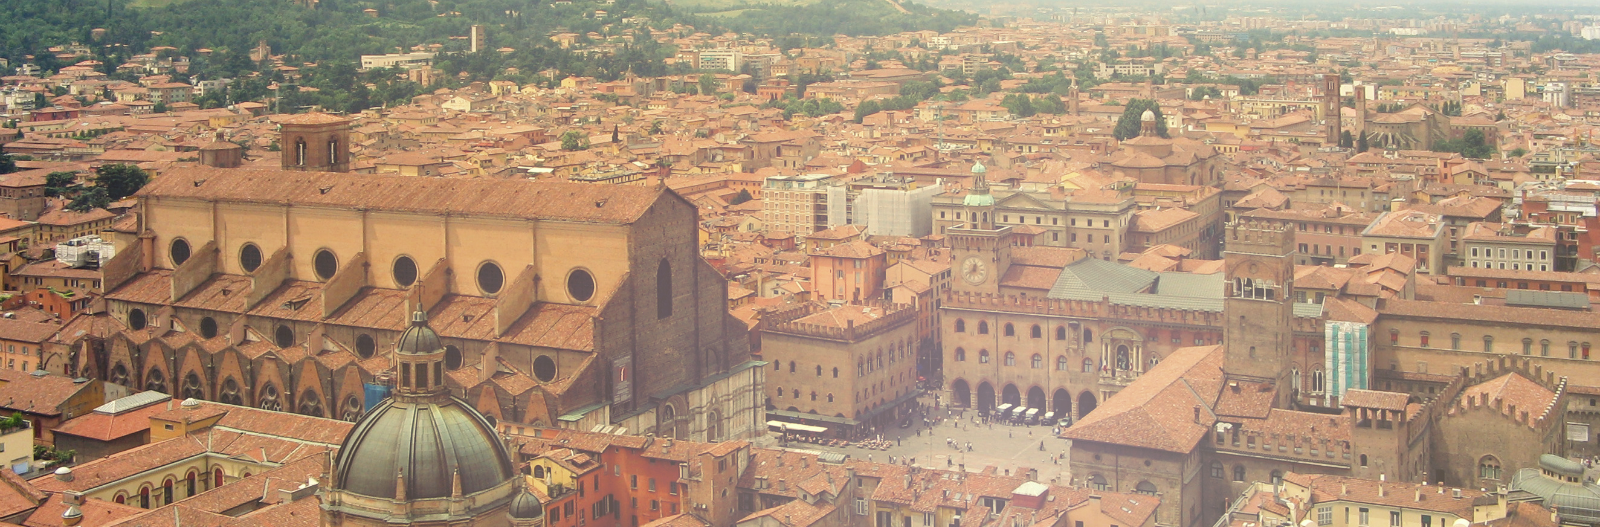
\includegraphics[width=\paperwidth,height=\paperheight,keepaspectratio]{./figures/bologna_strip.png}
    }
  }
}

\newgeometry{top=2.4cm,bottom=2.4cm,left=2.4cm,right=2.4cm}
\makeatletter

\begin{titlepage}
  \AddToShipoutPicture*{\BolognaBackgroundPic}
  
  \begin{center}
      \vspace*{1em}
      
\includegraphics[height=6em,keepaspectratio]{./figures/unibo_logo.png}\\
      %{\scshape\small Electric, Electronic and Information Engineering Department}\\[2em]
      \vspace{10em}
      {\sffamily\Huge \@title}\\[2em]
      {\sffamily Technical Report \TechReportNumber}\\[4em]
      {\sffamily\Large \@author}\\[2em]
      {\sffamily \@date}
      \vfill
      \begin{tikzpicture}[overlay, remember picture]
        \fill[black,opacity=0.5] (-12,-0.4) rectangle (12,-2.4);
        \node[color=white] at (-5,-1.4) {\sffamily {\Huge OR-Unibo}~~~Operational Research Group};
        % Twitter logo obtained from http://about.twitter.com/
        \node at (7,-1.4) {
\includegraphics[height=1.5em,keepaspectratio]{./figures/twitter_logo.png}};
        \node[color=white] at (8.75,-1.5) {\sffamily @OR\_Unibo};
      \end{tikzpicture}
  \end{center}
\end{titlepage}

\makeatother
\restoregeometry

% SET PAGE HEADER
\SetBgContents{\ORlogo}
\SetBgPosition{current page.north west}
\SetBgScale{0.4}
\SetBgAngle{0.0}

% PRINT THE TOC
\tableofcontents

% ALLOW ALIGN TO BREAK PAGES
% \allowdisplaybreaks

% YOUR TECH REPORT STARTS HERE

\chapter{Example of a chapter}\label{ch:example}
  
\section{Example of a section}\label{sec:first_example}
  
Ugly and futile: lean neck and thick hair and a stain of ink, a snail's
bed. Yet someone had loved him, borne him in her arms and in her heart.
But for her the race of the world would have trampled him underfoot,
a squashed boneless snail. She had loved his weak watery blood drained
from her own. Was that then real? The only true thing in life? His
mother's prostrate body the fiery Columbanus in holy zeal bestrode.
She was no more: the trembling skeleton of a twig burnt in the fire,
an odour of rosewood and wetted ashes. She had saved him from being
trampled underfoot and had gone, scarcely having been. A poor soul
gone to heaven: and on a heath beneath winking stars a fox, red reek
of rapine in his fur, with merciless bright eyes scraped in the earth,
listened, scraped up the earth, listened, scraped and scraped.

Sitting at his side Stephen solved out the problem. He proves by algebra
that Shakespeare's ghost is Hamlet's grandfather. Sargent peered askance
through his slanted glasses. Hockeysticks rattled in the lumberroom: the
hollow knock of a ball and calls from the field.

Across the page the symbols moved in grave morrice, in the mummery of
their letters, wearing quaint caps of squares and cubes. Give hands,
traverse, bow to partner: so: imps of fancy of the Moors. Gone too from
the world, Averroes and Moses Maimonides, dark men in mien and movement,
flashing in their mocking mirrors the obscure soul of the world, a
darkness shining in brightness which brightness could not comprehend.
  
\section{Another example of a section}\label{sec:second_example}

So saying, he stepped aside and wrote down a list of several books
treating of natural philosophy which he desired me to procure, and
dismissed me after mentioning that in the beginning of the following
week he intended to commence a course of lectures upon natural
philosophy in its general relations, and that M. Waldman, a fellow
professor, would lecture upon chemistry the alternate days that he
omitted.

I returned home not disappointed, for I have said that I had long
considered those authors useless whom the professor reprobated; but I
returned not at all the more inclined to recur to these studies in any
shape.  M. Krempe was a little squat man with a gruff voice and a
repulsive countenance; the teacher, therefore, did not prepossess me in
favour of his pursuits.  In rather a too philosophical and connected a
strain, perhaps, I have given an account of the conclusions I had come
to concerning them in my early years.  As a child I had not been
content with the results promised by the modern professors of natural
science.  With a confusion of ideas only to be accounted for by my
extreme youth and my want of a guide on such matters, I had retrod the
steps of knowledge along the paths of time and exchanged the
discoveries of recent inquirers for the dreams of forgotten alchemists.
Besides, I had a contempt for the uses of modern natural philosophy.
It was very different when the masters of the science sought
immortality and power; such views, although futile, were grand; but now
the scene was changed.  The ambition of the inquirer seemed to limit
itself to the annihilation of those visions on which my interest in
science was chiefly founded.  I was required to exchange chimeras of
boundless grandeur for realities of little worth.

Such were my reflections during the first two or three days of my
residence at Ingolstadt, which were chiefly spent in becoming
acquainted with the localities and the principal residents in my new
abode.  But as the ensuing week commenced, I thought of the information
which M. Krempe had given me concerning the lectures.  And although I
could not consent to go and hear that little conceited fellow deliver
sentences out of a pulpit, I recollected what he had said of M.
Waldman, whom I had never seen, as he had hitherto been out of town.

\section{A section referencing the bibliography}\label{sec:third_example}

The first two sections of this chapter contain random pieces from \citet{Shelley:1993:F} and \citet{Joyce:2003:U}. The rest of this section contains a piece from \citet{Zola:2004:G}.

Devant le buffet ouvert, Catherine réfléchissait.  Il ne restait qu'un
bout de pain, du fromage blanc en suffisance, mais à peine une
lichette de beurre; et il s'agissait de faire les tartines pour eux
quatre.  Enfin, elle se décida, coupa les tranches, en prit une
qu'elle couvrit de fromage, en frotta une autre de beurre, puis les
colla ensemble: c'était «le briquet», la double tartine emportée
chaque matin à la fosse.  Bientôt, les quatre briquets furent en rang
sur la table, répartis avec une sévère justice, depuis le gros du père
jusqu'au petit de Jeanlin.

Catherine, qui paraissait toute à son ménage, devait pourtant rêvasser
aux histoires que Zacharie racontait sur le maître-porion et la
Pierronne, car elle entrebâilla la porte d'entrée et jeta un coup
d'oeil dehors.  Le vent soufflait toujours, des clartés plus
nombreuses couraient sur les façades basses du coron, d'où montait une
vague trépidation de réveil.  Déjà des portes se refermaient, des
files noires d'ouvriers s'éloignaient dans la nuit.  Était-elle bête,
de se refroidir, puisque le chargeur à l'accrochage dormait bien sûr,
en attendant d'aller prendre son service, à six heures! Et elle
restait, elle regardait la maison, de l'autre côté des jardins.  La
porte s'ouvrit, sa curiosité s'alluma.  Mais ce ne pouvait être que la
petite des Pierron, Lydie, qui partait pour la fosse.  

% BIBLIOGRAPHY
\bibliographystyle{plainnat}
\bibliography{report}
\end{document}